\hspace{24pt}

In Section~\ref{sec:result}, we have seen that the best performance of the zh-ja NMT system can be achieved by utilizing Jieba \& Janome as the tokenization method and the joint embedding as an additional feature in the Transformer model. Based on the promising performance of the models, we will further examine the translation results produced by the best model and try to explain the reasons for its improved translation in Section~\ref{sec:case_study}. In addition, we will compare the joint embedding with the semantic embedding in Section~\ref{sec:analysis} to further analyze the advantages that the joint embedding provides over traditional embedding.

\section{Case Study} \label{sec:case_study}

We compare the translation results using joint embedding with those using semantic embedding. The results show that the use of joint embedding is superior to that of semantic embedding in four aspects.

\vspace{0.4cm}
\begin{table}[h]
    \centering
    \begin{CJK}{UTF8}{gbsn}
        \begin{tabularx}{\textwidth}{p{1.2cm}b}\toprule
            Source & 使用有机溶剂的溶剂提取法作为物质的分离手段被广泛利用。 \\
        \end{tabularx}
    \end{CJK}

    \begin{CJK}{UTF8}{ipxm}
        \begin{tabularx}{\textwidth}{p{1.2cm}b}
            Target & 有機溶媒を用いた溶媒抽出法は物質の分離手段として広く利用されている。 \\
            Semantic & 有機溶媒を用いた溶媒抽出法は物質の分離手段として広く\underline{用いされ}ている。 \\
            Joint & 有機溶媒を用いた溶媒抽出法は物質の分離手段として広く\underline{利用され}ている。 \\\midrule
        \end{tabularx}
    \end{CJK}

    \begin{CJK}{UTF8}{gbsn}
        \begin{tabularx}{\textwidth}{p{1.2cm}b}
            Source & 在本章中,将分布式组件间进行通信的中间件与Dragon进行比较。 \\
        \end{tabularx}
    \end{CJK}

    \begin{CJK}{UTF8}{ipxm}
        \begin{tabularx}{\textwidth}{p{1.2cm}b}
            Target & 本章では,分散コンポーネント間通信を行うミドルウェアとDragonを比較する. \\
            Semantic & 本章では,\underline{分散コンポーネント間}でを行うミドルウェアとDragonを比較する. \\
            Joint & 本章では,\underline{分散コンポーネント間通信}を行うミドルウェアとDragonを比較する. \\\midrule
        \end{tabularx}
    \end{CJK}

    \begin{CJK}{UTF8}{gbsn}
        \begin{tabularx}{\textwidth}{p{1.2cm}b}
            Source & LearnAR从背景知识B和观测结果O中获得行动规则的集合γ的集合H。 \\
        \end{tabularx}
    \end{CJK}

    \begin{CJK}{UTF8}{ipxm}
        \begin{tabularx}{\textwidth}{p{1.2cm}b}
            Target & LearnARは,背景知識Bと観測結果Oより行動規則の集合γ\underline{の集合を}獲得する. \\
            Semantic & LearnARは\underline{背景背景知識}Bと観測結果Oから\underline{行動ルール}の集合γの集合H獲得する. \\
            Joint & LearnARは,\underline{背景知識}Bと観測結果Oから\underline{行動規則}の集合γ\underline{の集合H}獲得する. \\\midrule
        \end{tabularx}
    \end{CJK}

    \caption{Case Study - Retention of correct words}
    \label{tab:case_study1}
\end{table}

\begin{CJK}{UTF8}{ipxm}
    Table~\ref{tab:case_study1} compares the results of the two translations in terms of their ability to preserve correct words. In the first example, ``利用され'' (be used) is correctly translated by the joint embedding, while semantic embedding produces the ungrammatical string ``用いされ'', which is perhaps an unfortunate combination of ``利用され'' and an alternative translation ``用いられ''.
In the second example, ``分散コンポーネント間通信'' (communication between distributed components) is correctly translated by the joint embedding, and the semantic embedding omits ``通信'' (communication).  The third example demonstrates that both the semantic and joint embedding can correctly retain the symbol $H$ even though it is missing from the target sentence, however the joint embedding translation is overall closer to the target.  In fact, at least for these three examples, the joint embedding translation is consistently more fluent than those of the semantic embedding. 
\end{CJK}

\vspace{0.4cm}
\begin{table}[h]
    \centering

    \begin{CJK}{UTF8}{gbsn}
        \begin{tabularx}{\textwidth}{p{1.2cm}b}\toprule
            Source & 构成这些乐曲时在可能范围里保证变化丰富。 \\
        \end{tabularx}
    \end{CJK}

    \begin{CJK}{UTF8}{ipxm}
        \begin{tabularx}{\textwidth}{p{1.2cm}b}
            Target & これらの楽曲は,可能な範囲でバリエーションが豊かになるように構成されている. \\
            Semantic & これらの楽曲を,豊かな範囲で\underline{変化}が豊かになる.にしされている. \\
            Joint & これらの楽曲を,可能な範囲で\underline{バリエーション}が豊かになるように構成されている. \\\midrule
        \end{tabularx}
    \end{CJK}

    \begin{CJK}{UTF8}{gbsn}
        \begin{tabularx}{\textwidth}{p{1.2cm}b}
            Source & 铝焊接烟气的特性 \\
        \end{tabularx}
    \end{CJK}

    \begin{CJK}{UTF8}{ipxm}
        \begin{tabularx}{\textwidth}{p{1.2cm}b}
            Target & アルミニウム溶接ヒュームの物性 \\
            Semantic & アルミニウム溶接\underline{煙}の特性 \\
            Joint & アルミニウム溶接\underline{ヒューム}の特性 \\\midrule
        \end{tabularx}
    \end{CJK}
    \caption{Case Study - Utilization of English loanwords}
    \label{tab:case_study2}
\end{table}

\begin{CJK}{UTF8}{ipxm}
    Table~\ref{tab:case_study2} demonstrates the ability of joint embedding to utilize English loanwords.  Loan-words from English and occasionally German or other western languages play in important role in modern Japanese and occur with significant frequency in scientific technical writing.  Thus a natural translation of Chinese into Japanese is likely to include some of these loanwords, easily spotted due to the convention of using katakana to write them.  Here we show a couple of examples in which the joint embedding uses such a loanword while the semantic embedding does not.  In the first example we focus on the translation of
\end{CJK}\begin{CJK}{UTF8}{gbsn}the ``变化'' in the Chinese \mbox{``变化丰富''}.
Which is translated as''\variation'' by the target and semantic embedding,
\end{CJK}\begin{CJK}{UTF8}{ipxm}
but as ``変化'' by the joint embedding.
変化 is a common word shared by Chinese and Japanese, which depending on context might be translated into English as: ``change'', ``alteration'', ``inflection'', or ``variation''.  ``variation'' happens to be a word which has been borrowed into the Japanese language using the katakana spelling
\end{CJK}\begin{CJK}{UTF8}{ipxm}''\variation''.  Although partially overlapping in meaning with ``変化'',\enspace\variation\ is more specific and in particular tends to have a positive meaning in Japanese, which matches the positive connotation of
\end{CJK}\begin{CJK}{UTF8}{gbsn}''丰富'' (abundant) in the source.
\end{CJK}\begin{CJK}{UTF8}{ipxm}These factors explain why \variation\ was selected in the target, instead of directly copying 変化 from the source.  The second example involves the translation of
\end{CJK}\begin{CJK}{UTF8}{gbsn}''烟气'' to either
\end{CJK}\begin{CJK}{UTF8}{ipxm}``ヒューム'' or ``煙''.
ヒューム is the loanword ``fume'' borrwed from English, while 煙 is the general Japanese word for smoke.  In informal speech a Japanese speaker might use ``煙'' to describe any smoke-like phenonemon (even steam), but the target sentence selects ヒューム, as a more specific and technically correct word in the source sentence context of welding.  The joint embedding also selects ヒューム, but the semantic embedding selects ``煙''.
Interestingly, in both of these examples the semantic translation more or less directly copies the Chinese word to produce a Japanese translation which is arguably not far off the mark semantically, but the word choice of the joint embedding is much preferred.
\end{CJK}

\vspace{0.4cm}
\begin{table}[h]
    \centering

    \begin{CJK}{UTF8}{gbsn}
        \begin{tabularx}{\textwidth}{p{1.2cm}b}\toprule
            Source & RMCPRGIGCenter和RMCPRGIGTransceiver使用C语言安装,在二者间的通信中和RemoteGIG同样使用TCP/IP上的RMCP。 \\
        \end{tabularx}
    \end{CJK}

    \begin{CJK}{UTF8}{ipxm}
        \begin{tabularx}{\textwidth}{p{1.2cm}b}
            Target & RMCPRGIGCenterとRMCPRGIGTransceiverはC言語で実装し,両者間の通信にはRemoteGIGと同様にTCP/IP上のRMCPを用いた. \\
            Semantic & RMCPRGIGCenterと\underline{RMCPRGIGTranscei}はC言語を実装し,両者間通信通信で\underline{TCPTCP}と同様にTCP/IPででRMCPを用いるて. \\
            Joint & RMCPRGIGCenterと\underline{RMCPRGIGTransceiver}をC言語を実装し,両者間の通信においては\underline{RemoteGIG}と同様にTCP/IP上でRMCPを用いた. \\\midrule
        \end{tabularx}
    \end{CJK}

    \begin{CJK}{UTF8}{gbsn}
        \begin{tabularx}{\textwidth}{p{1.2cm}b}
            Source & 另一方面,GUIServer和GUIClient是用Java语言进行安装。 \\
        \end{tabularx}
    \end{CJK}

    \begin{CJK}{UTF8}{ipxm}
        \begin{tabularx}{\textwidth}{p{1.2cm}b}
            Target & 一方,GUIServerとGUIClientはJava言語で実装した. \\
            Semantic & 一方,\underline{GUISverver}や\underline{GUIIClient}はJava言語で実装した. \\
            Joint & 一方,\underline{GUIServer}と\underline{GUIClient}はJava言語で実装した. \\\midrule
        \end{tabularx}
    \end{CJK}

    \caption{Case Study - Preservation of English acronyms and technical jargon}
    \label{tab:case_study3}
\end{table}

\begin{CJK}{UTF8}{ipxm}
    Table~\ref{tab:case_study3} demonstrates the ability of joint embedding to cope with Chinese or Japanese text including English acronyms and technical jargon verbatim.  When English words are present, semantic embedding often produces strange translations.
It will lose English words, generate the wrong English words and grammar.  Fortunately, joint embedding does not exhibit these problems.
%% PH  為什麼 semantic embedding會有這麼奇怪的結果 像"GUIClient"-->"GUIIClient"??
\end{CJK}

\begin{table}[h]
    \centering

    \begin{CJK}{UTF8}{gbsn}
        \begin{tabularx}{\textwidth}{p{1.2cm}b}\toprule
            Source & 微小粒子测量装置的比较试验 \\
        \end{tabularx}
    \end{CJK}

    \begin{CJK}{UTF8}{ipxm}
        \begin{tabularx}{\textwidth}{p{1.2cm}b}
            Target & 微小粒子測定装置の比較試験 \\
            Semantic & 微小粒子\underline{計測}装置の比較\underline{実験} \\
            Joint & 微小粒子\underline{測定}装置の比較\underline{試験} \\\midrule
        \end{tabularx}
    \end{CJK}

    \begin{CJK}{UTF8}{gbsn}
        \begin{tabularx}{\textwidth}{p{1.2cm}b}
            Source & 胃运动机能和NERD的病状的关连性的相关讨论 \\
        \end{tabularx}
    \end{CJK}

    \begin{CJK}{UTF8}{ipxm}
        \begin{tabularx}{\textwidth}{p{1.2cm}b}
            Target & 胃運動機能とNERDの病態との関連性に関する検討 \\
            Semantic & 胃運動機能とNERDの病態\underline{の}の関連性に関する\underline{議論} \\
            Joint & 胃運動機能とNERDの病態\underline{と}の関連性に関する\underline{検討} \\\midrule
        \end{tabularx}
    \end{CJK}

    \begin{CJK}{UTF8}{gbsn}
        \begin{tabularx}{\textwidth}{p{1.2cm}b}
            Source & 此外,用100对属性数进行了均等化。 \\
        \end{tabularx}
    \end{CJK}

    \begin{CJK}{UTF8}{ipxm}
        \begin{tabularx}{\textwidth}{p{1.2cm}b}
            Target & また,属性数を100で均一化した. \\
            Semantic & また,属性数を100で\underline{均等化}した. \\
            Joint & また,属性数を100で\underline{均一化}した. \\\midrule
        \end{tabularx}
    \end{CJK}

    \caption{Case Study - More appropriate word selection}
    \label{tab:case_study4}
\end{table}

\begin{CJK}{UTF8}{ipxm}
    Table~\ref{tab:case_study4} shows that joint embedding will select more precise words for translation.
In the first example, ``測定装置'' is commonly used to indicate the ``measuring instrument'' meaning of the source
\end{CJK}\begin{CJK}{UTF8}{gbsn}''测量装置'',
\end{CJK}\begin{CJK}{UTF8}{ipxm}
while ``計測'' is more often used independently to indicate ``measurement'', that is, using instruments to measure. In addition, joint embedding also correctly maps the Chinese word
\end{CJK}\begin{CJK}{UTF8}{gbsn}``试验'' (test) to its Japanese counterpart
\end{CJK}\begin{CJK}{UTF8}{ipxm}``試驗'' (test) rather than ``実験'' (experiment).
The second example involves the whether to translate the Chinese word
\end{CJK}\begin{CJK}{UTF8}{gbsn}''讨论'',
\end{CJK}\begin{CJK}{UTF8}{ipxm}
to the Japanese word ``検討'' or ``議論''.
\end{CJK}\begin{CJK}{UTF8}{gbsn} Depending on context, 讨论 can mean ``discussion'' and in those case might be translated as
\end{CJK}\begin{CJK}{UTF8}{ipxm}``議論'' which in Japanese means ``discussion'' or ``debate''.
Howver in the source sentence
\end{CJK}\begin{CJK}{UTF8}{gbsn}
讨论, is used in the sense of ``thoughtful consideration'', which is more appropriately translated as
\end{CJK}\begin{CJK}{UTF8}{ipxm}
検討, found in the target and joint embedding translation, but not the semantic embedding.
The third example involves whether to directly copy the Chinese word
\end{CJK}\begin{CJK}{UTF8}{gbsn}''均等化''
as is in the Japanese translation, since
\end{CJK}\begin{CJK}{UTF8}{ipxm}''均等化'' is a valid Japanese word with similar meaning,
or to instead use an alternative Japanese word \mbox{``均一化''}.
Both words are technical in nature, but joint embedding selection ``均一化'' concurs with the target sentence, so it may be considered preferable to simply copying \mbox{均等化} as done by the semantic embedding.
%%In the third example, it is also better to use ``均一化'' (regularization) than ``均等化'' (equalization) in the context.
%% 我覺得  均一化 ≝ regularization  ≠  均等化 ≝ equalization  不一定成立,  也許 均一化 ≈ 均等化.
\end{CJK}

\section{Embedding Analysis} \label{sec:analysis}

We applied four analysis methods to compare joint embedding and semantic embedding. In all four analyses, joint embedding preserves the properties that semantic embedding should have and even outperforms semantic embedding.

\subsection{Analogical Reasoning} \label{sec:analysis_analogy}

The joint embedding can also produce correct answers in the analogical reasoning task.  We found that the answers obtained from joint embedding received higher confidence values on average in both Chinese (Table~\ref{tab:analysis_analogy1}) and Japanese (Table~\ref{tab:analysis_analogy2}). 

\begin{table}[h]
    \centering
    \begin{CJK}{UTF8}{gbsn}
        \begin{tabularx}{\textwidth}{lllbb}
            \toprule
            \multicolumn{3}{c}{Input} & \multicolumn{2}{c}{Output ($b*$)} \\
            \cmidrule(lr){1-3} \cmidrule(lr){4-5} $a$ & $a*$ & $b$ & Semantic & Joint \\\midrule
            \vspace{0.2cm} 东京 (Tokyo) & 日本 (Japan) & 北京 (Beijing) & 中国 (China) \newline ($p=0.492$) & 中国 (China) \newline ($\bm{p=0.531}$) \\
            \vspace{0.2cm} 长期 (long-term) & 三年 (3 years) & 短期 (short-term) & 一年 (1 year) \newline ($p=0.379$) & \mbox{两周} (\mbox{2 weeks}) \newline ($\bm{p=0.387}$) \\
            进口 (import) & 买入 (buy) & 出口 (export) & 卖出 (sell) \newline ($p=0.364$) & 卖出 (sell) \newline ($\bm{p=0.442}$)\\\bottomrule
        \end{tabularx}
    \end{CJK}
    \caption{Analogical Reasoning in Chinese}
    \label{tab:analysis_analogy1}
\end{table}

\begin{table}[h]
    \centering
    \begin{CJK}{UTF8}{ipxm}
        \begin{tabularx}{\textwidth}{lllbb}
            \toprule
            \multicolumn{3}{c}{Input} & \multicolumn{2}{c}{Output ($b*$)} \\
            \cmidrule(lr){1-3} \cmidrule(lr){4-5} $a$ & $a*$ & $b$ & Semantic & Joint \\\midrule
            \vspace{0.2cm} 男性(male) & 女性 (female) & 父親 (father) & \mbox{母親} (mother) \newline ($p=0.487$) & \mbox{母親} (mother) \newline ($\bm{p=0.508}$) \\
            \vspace{0.2cm} 長期 (long-term) & 年 (year) & 短期 (short-term) & 月 (month) \newline ($p=0.550$) & 月 (month) \newline ($\bm{p=0.570}$) \\
            左右(left-right) & 前後 (front-rear) & 水平 (horizontal) & \mbox{垂直} (\mbox{vertical}) \newline ($\bm{p=0.432}$) & \mbox{垂直} (\mbox{vertical}) \newline ($p=0.402$) \\\bottomrule
        \end{tabularx}
    \end{CJK}
    \caption{Analogical Reasoning in Japanese}
    \label{tab:analysis_analogy2}
\end{table}

\subsection{Outlier Detection} \label{sec:analysis_outlier}

\begin{CJK}{UTF8}{gbsn}    
    Joint embedding can answer outlier detection problems as well as semantic embedding, and sometimes gives better answers. For example, in the second case of Table~\ref{tab:analysis_outlier1}, the joint embedding answers correctly, while semantic embedding answers incorrectly.
\end{CJK}

\begin{table}[h]
    \centering
    \begin{CJK}{UTF8}{gbsn}
        \begin{tabularx}{\textwidth}{bll}
            \toprule
            \multirow{2.5}{*}{Word Cluster} & \multicolumn{2}{c}{Outlier (Output)} \\
            \cmidrule(lr){2-3} {} & Semantic & Joint \\\midrule

            鸟 (birds), 狗 (dogs), 猫 (cats), 花 (flowers) & \vspace{0.25cm} 花 (flowers) & 花 (flowers) \\

            可行(feasible), 不行 (not OK), 行 (OK), \mbox{可以}~(can/OK) & \vspace{0.25cm} 可以 (can/OK) & 不行 (not OK) \\

            \mbox{广岛} (Hiroshima), \mbox{名古屋} (Nagoya), \mbox{爱知}(Aichi), 上海 (Shanghai, only this one is in China) & 上海 (Shanghai) & 上海 (Shanghai)\\\bottomrule
        \end{tabularx}
    \end{CJK}
    \caption{Outlier Detection in Chinese}
    \label{tab:analysis_outlier1}
\end{table}

\begin{table}[h]
    \centering
    \begin{CJK}{UTF8}{ipxm}
        \begin{tabularx}{\textwidth}{bll}
            \toprule
            \multirow{2.5}{*}{Word Cluster} & \multicolumn{2}{c}{Outlier (Output)} \\
            \cmidrule(lr){2-3} {} & Semantic & Joint \\\midrule
            生み (birth), 創造 (creation), 作る (making), 破壊 (destruction) & \vspace{0.25cm} 破壊 (destruction) & 破壊 (destruction) \\
            普通 (normal), 一般 (general), 通常 (normal), 異常 (abnormal) & \vspace{0.25cm} 異常 (abnormal) & 異常 (abnormal) \\
            \mbox{平成} (Heisei era), \mbox{昭和} (Showa era), \mbox{大正}~(Taisho era), \mbox{明治} (Meiji era), \mbox{京都}~(\mbox{Kyoto}) & 京都 (Kyoto) & 京都 (Kyoto) \\\bottomrule
        \end{tabularx}
    \end{CJK}
    \caption{Outlier Detection in Japanese}
    \label{tab:analysis_outlier2}
\end{table}

\vspace{0.4cm}
\begin{figure}[h!]
    \begin{CJK}{UTF8}{gbsn}
    \centering
    \begin{subfigure}[b]{0.46\textwidth}
        \centering
        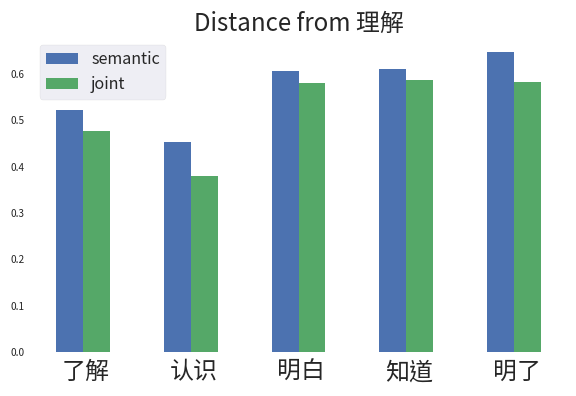
\includegraphics[width=\textwidth]{../images/similarity_zh1.png}
        \caption{Similarity distances between ``理解'' (comprehend) and its synonyms are reduced in the joint embedding}
        \label{fig:similarity_zh1}
    \end{subfigure}
    \hspace{2em}
    \begin{subfigure}[b]{0.46\textwidth}
        \centering
        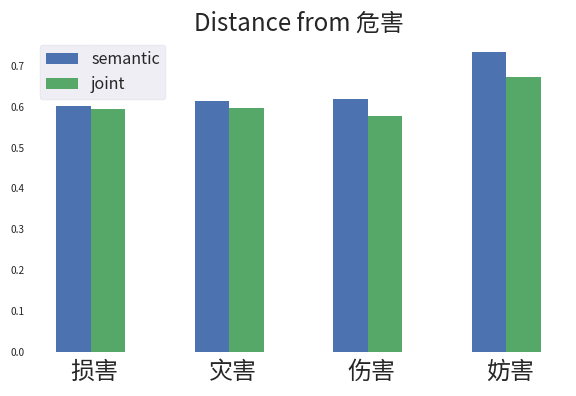
\includegraphics[width=\textwidth]{../images/similarity_zh2.png}
        \caption{Similarity distances between ``危害'' (jeopardize) and its synonyms are reduced in the joint embedding}
        \label{fig:similarity_zh2}
    \end{subfigure}
    %%
    \begin{subfigure}[b]{0.46\textwidth}
        \centering
        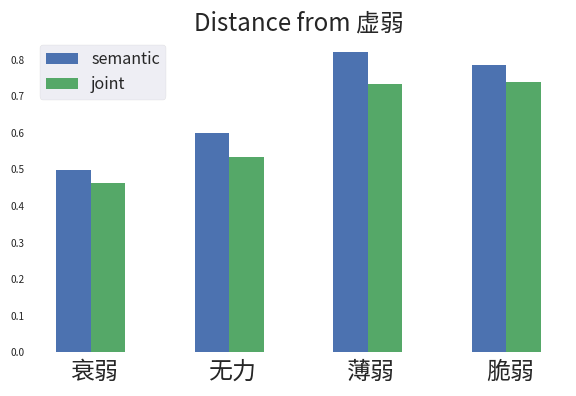
\includegraphics[width=\textwidth]{../images/similarity_zh3.png}
        \caption{Similarity distances between ``虛弱'' (weak) and its synonyms are reduced in the joint embedding}
        \label{fig:similarity_zh3}
    \end{subfigure}
    \hspace{2em}
    \begin{subfigure}[b]{0.46\textwidth}
        \centering
        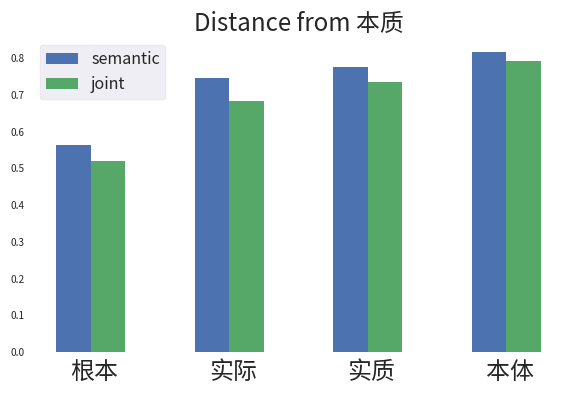
\includegraphics[width=\textwidth]{../images/similarity_zh4.png}
        \caption{Similarity distances between ``本质'' (essence) and its synonyms are reduced in the joint embedding}
        \label{fig:similarity_zh4}
    \end{subfigure}
    \caption{Similarity distances between synonyms in Chinese}
	\label{fig:similarity_zh}
\end{CJK}
\end{figure}

\subsection{Word Similarity} \label{sec:analysis_similarity}
\begin{CJK}{UTF8}{gbsn}
    The similarity distance between synonyms is not only preserved but also shortened. This finding indicates the joint embedding not only protects but also enhances the semantics by adding phonetic information. Figure~\ref{fig:similarity_zh} shows that the similarity distances of Chinese synonyms are shortened in the joint embedding. For example, Figure~\ref{fig:similarity_zh1} shows that the distance between ``了解 (understand), 认识 (recognize), 明白 (realize), 知道 (know), 明了 (clearly understand)'' and ``理解 (comprehend)'' are reduced in the joint embedding.

    % ``了解 (understand), 认识 (recognize), 明白 (realize), 知道 (know), 明了 (clearly understand)'', ``理解 (comprehend)'' 
    
    % ``损害 (harm), 灾害 (calamity), 伤害 (injure), 妨害 (impair)'', ``危害 (jeopardize)''
    
    % ``衰弱 (feeble), 无力 (powerless), 薄弱 (frail), 脆弱 (fragile)', ``虚弱 (weak)''. 
    
    % ``根本 (fundamental), 实际 (reality), 实质 (substance), 本体 (ontology)'', ``本质 (essence)''.
\end{CJK}

\begin{CJK}{UTF8}{ipxm}
    Similarly, the similarity distances of Japanese synonyms are also shortened with the use of joint embedding. Especially in Japanese, sometimes hiragana and kanji are used interchangeably. For example, in Figure~\ref{fig:similarity_ja4}, ``また'' and ``又 (また)'' have the pronunciation and meaning (``again''). The joint embedding can find the relationship between them and reduce their distance significantly.
\end{CJK}

\vspace{0.4cm}
\begin{CJK}{UTF8}{ipxm}
    \begin{figure}[h]
        \centering
        \begin{subfigure}[b]{0.46\textwidth}
            \centering
            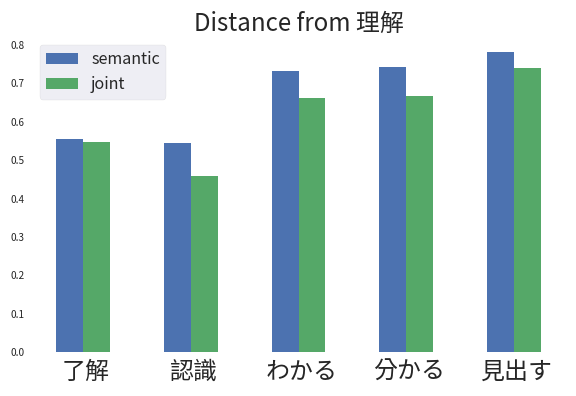
\includegraphics[width=\textwidth]{../images/similarity_ja1.png}
            \caption{Similarity distances between ``理解'' (comprehend) and its synonyms.}
            \label{fig:similarity_ja1}
        \end{subfigure}
        \hspace{2em}
        \begin{subfigure}[b]{0.46\textwidth}
            \centering
            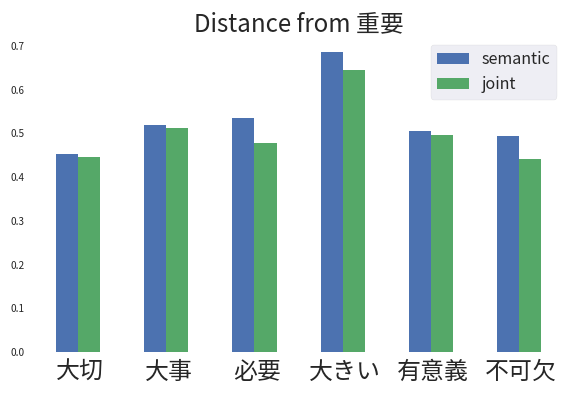
\includegraphics[width=\textwidth]{../images/similarity_ja2.png}
            \caption{Similarity distances between ``重要''' (important) and its synonyms.}
            \label{fig:similarity_ja2}
        \end{subfigure}
        %%
        \begin{subfigure}[b]{0.46\textwidth}
            \centering
            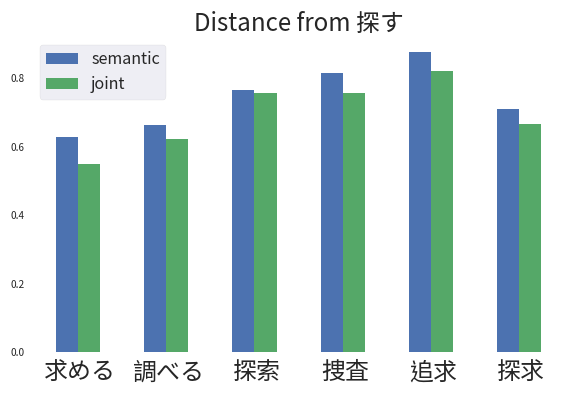
\includegraphics[width=\textwidth]{../images/similarity_ja3.png}
            \caption{Similarity distances between ``探す'' (seek) and its synonyms.}
            \label{fig:similarity_ja3}
        \end{subfigure}
        \hspace{2em}
        \begin{subfigure}[b]{0.46\textwidth}
            \centering
            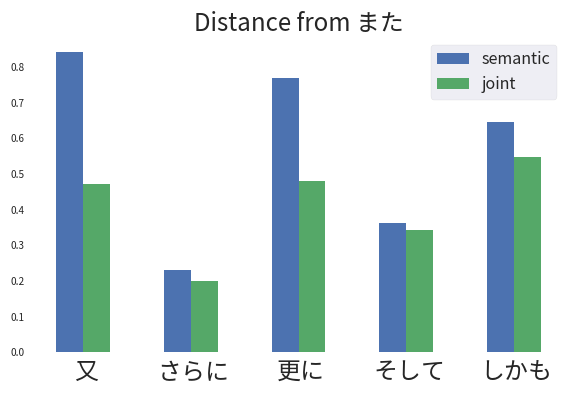
\includegraphics[width=\textwidth]{../images/similarity_ja4.png}
            \caption{Similarity distances between ``\mbox{また}'' (again) and its synonyms.}
            \label{fig:similarity_ja4}
        \end{subfigure}
        \caption{Similarity distances between synonyms in Japanese.  In all cases joint embedding assigns shorter distances.}
        \label{fig:similarity_ja}
    \end{figure}
    \end{CJK}

\subsection{Homonym and Heteronym} \label{sec:analysis_homonym_heteronym}

We also found encouraging results from tests on homonyms and heteronyms. The higher correlation between the homonym vectors indicates that the joint embedding can help the model be robust against noise (typographical errors).  The increase in the similarity distance between heteronyms implies that the phonetic information effectively separates them, which is a sign of semantic enhancement.

\begin{figure}[t]
    \centering
    \begin{subfigure}[b]{0.49\textwidth}
        \centering
        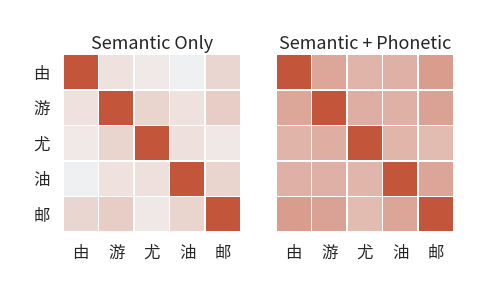
\includegraphics[width=\textwidth]{../images/corr_zh1.png}
        \caption{Pearson correlation between characters pronounced\enspaceㄧㄡˊ (yóu).}
        \label{fig:corr_zh1}
    \end{subfigure}
    \hfill
    \begin{subfigure}[b]{0.49\textwidth}
        \centering
        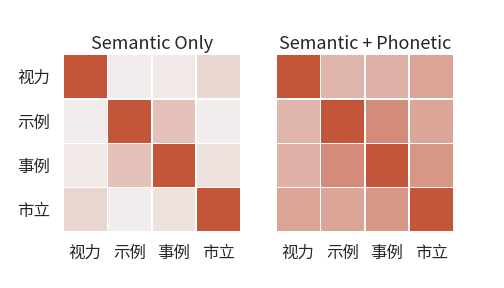
\includegraphics[width=\textwidth]{../images/corr_zh2.png}
        \caption{Pearson correlation between words pronounced\enspaceㄕˋ ㄌㄧˋ (shì lì).}
        \label{fig:corr_zh2}
    \end{subfigure}
    \begin{subfigure}[b]{0.49\textwidth}
        \centering
        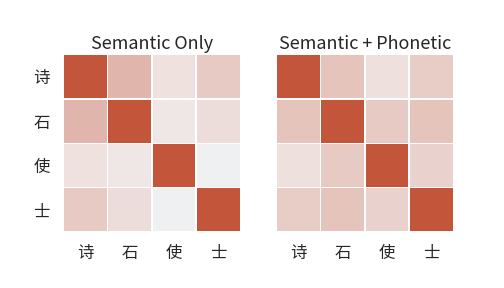
\includegraphics[width=\textwidth]{../images/corr_zh3.png}
        \caption{Pearson correlation between characters pronounced\enspaceㄕ (shi).}
        \label{fig:corr_zh3}
    \end{subfigure}
    \caption{Pearson correlation between homonyms in Chinese.  In all three cases shown, the correlation between homonyms or near homonyms is greater in the joint embedding than the semantic embedding.}
    \label{fig:corr_zh}
\end{figure}

\subsubsection{Homonym}

In Figure~\ref{fig:corr_zh}, we examine the correlations between Chinese homonyms in three scenarios:
the correlation of homophonic characters (Figure~\ref{fig:corr_zh1}), the correlation of homophonic words (Figure~\ref{fig:corr_zh2}), and the correlation of words with the same pronunciation except for having different tones (Figure~\ref{fig:corr_zh3}).
The results show that the correlation of these homonyms and near homonyms is greater under the joint embedding.

In Figure~\ref{fig:corr_ja}, we also examine the correlations between Japanese homonyms in three scenarios. Since there are no tones in Japanese, we tested the homonyms with single syllable (Figure~\ref{fig:corr_ja1}), homonyms with two syllables (Figure~\ref{fig:corr_ja2}), and homophonic words (Figure~\ref{fig:corr_ja3}). All the results have shown that joint embedding can effectively improve the correlation between Japanese homonymns.

\begin{figure}[t]
    \centering
    \begin{subfigure}[b]{0.49\textwidth}
        \centering
        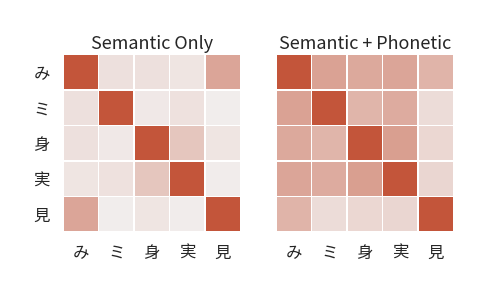
\includegraphics[width=\textwidth]{../images/corr_ja1.png}
        \caption{Pearson correlation between characters pronounce (mi).}
        \label{fig:corr_ja1}
    \end{subfigure}
    \hfill
    \begin{subfigure}[b]{0.49\textwidth}
        \centering
        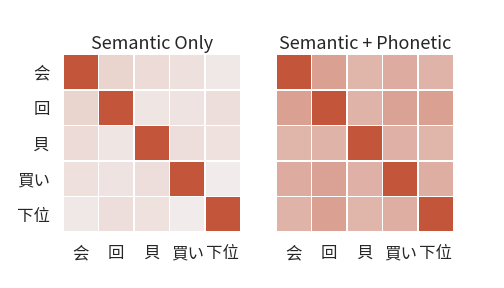
\includegraphics[width=\textwidth]{../images/corr_ja2.png}
        \caption{Pearson correlation between characters and words pronounced (kai).}
        \label{fig:corr_ja2}
    \end{subfigure}
    \begin{subfigure}[b]{0.49\textwidth}
        \centering
        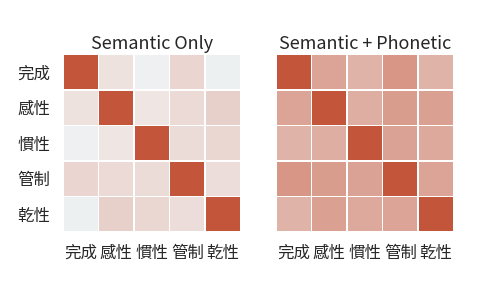
\includegraphics[width=\textwidth]{../images/corr_ja3.png}
        \caption{Pearson correlation between words pronounced (kansei).}
        \label{fig:corr_ja3}
    \end{subfigure}
    \caption{Pearson correlation between homonyms in Japanese.  In any cases the correlation is higher under joint embedding.}
    \label{fig:corr_ja}
\end{figure}

\newpage

\subsubsection{Heteronym}

In Table~\ref{tab:analysis_heteronym1}, we compare the similarity distance between Chinese heteronyms.  The first example is ``長'' meaning ``length'' when pronounced one way (ㄔㄤˊ) and growth when pronounced another way (ㄓㄤˇ).  The second example is ``樂'', meaning joyful (ㄌㄜˋ) or musical sound (ㄩㄝˋ).  The third example ``中'' stands for middle (ㄓㄨㄥ) or hitting a target (ㄓㄨㄥˋ) respectively. In all three examples, the similarity distances are greater in the joint embedding, which implies that the phonetic information can help distinguish between heteronyms.

\vspace{0.5cm}
\begin{table}[h]
    \centering
        \begin{tabularx}{\textwidth}{bbbb}
            \toprule
            \multirow{2.5}{*}{A} & \multirow{2.5}{*}{B} & \multicolumn{2}{c}{Similarity Distance} \\
            \cmidrule(lr){3-4} {} & {} & Semantic & Joint \\\midrule
            長 (ㄔㄤˊ) 度 & 長 (ㄓㄤˇ) 大 & 0.826 & \textbf{0.853} \\
            樂 (ㄌㄜˋ) 趣 & 音樂 (ㄩㄝˋ) & 0.636 & \textbf{0.682} \\
            中 (ㄓㄨㄥ) 午 & 中 (ㄓㄨㄥˋ) 毒 & 0.842 & \textbf{0.866} \\\bottomrule
        \end{tabularx}
    \caption{Similarity distance between heteronyms in Chinese}
    \label{tab:analysis_heteronym1}
\end{table}

\newpage

\begin{CJK}{UTF8}{ipxm}
    In Table~\ref{tab:analysis_heteronym2}, the same advantage also appears in Japanese. We have compared the different pronunciations and meanings of ``生'', a character notorious for having so many distinct readings.  We compared the readings (なま) ``raw'' , (しょう) ``life'' , (う) ``birth'' , and (き) ``unprocessed''. All the results show that joint embedding can increase the similarity distance between them.
\end{CJK}

\vspace{0.4cm}    
\begin{table}[h]
    \centering
    \begin{CJK}{UTF8}{ipxm}
        \begin{tabularx}{\textwidth}{bbbb}
            \toprule
            \multirow{2.5}{*}{A} & \multirow{2.5}{*}{B} & \multicolumn{2}{c}{Similarity Distance} \\
            \cmidrule(lr){3-4} {} & {} & Semantic & Joint \\\midrule
            生 (なま) & 一生 (しょう) & 0.879 & \textbf{0.889} \\
            生 (なま) & 生 (う) む & 0.830 & \textbf{0.839} \\
            生 (なま) & 生 (き) 地 & 0.769 & \textbf{0.867} \\\bottomrule
        \end{tabularx}
    \end{CJK}
    \caption{Similarity distance between heteronyms in Japanese}
    \label{tab:analysis_heteronym2}
\end{table}

\begin{CJK}{UTF8}{ipxm}
    There is a special feature in Japanese where many kanji are assigned a pair of readings; one originally derived from Chinese called on-yomi (音読み) and another of more purely Japanese origin (i.e.\ not from Chinese) called kun-yomi (訓読み).  In general the on-yomi and kun-yomi pronunciations of characters are entirely unrelated, but the meaning is usually very close.  In many cases, the kun-yomi pronunication is used when the word is used along, while the on-yomi is used as an element to form compound words.  A situation roughly analogous to what English might look like if we used a special water symbol to write both ``water'' and ``hydro''.  

We examined the (on-yomi, kun-yomi) pairs in Table~\ref{tab:analysis_heteronym3}. For example, when ``土'' is pronounced as ``つち'' or ``と'', it means soil; when ``海'' is pronounced as ``うみ'' or ``かい'', it means sea; when ``時'' is pronounced as ``とき'' or ``じ'', it means time.  Despite having completely different pronunciation, these semantically close (on-yomi,kun-yomi) pairs are closer to each other under the joint embedding.
% The joint embedding is not affected much by heteronyms and correctly reduces the distance of these words; the reason is possibly due to the well-balanced between semantics and phonetics.
%%PH 我怕這個只是cherry pick的效果
%%PH "well-balanced between semantics and phonetics." 是不是你隨便寫的?
\end{CJK}

\vspace{0.4cm}    
\begin{table}[h]
    \centering
    \begin{CJK}{UTF8}{ipxm}
        \begin{tabularx}{\textwidth}{bbbb}
            \toprule
            \multirow{2.5}{*}{A} & \multirow{2.5}{*}{B} & \multicolumn{2}{c}{Similarity Distance} \\
            \cmidrule(lr){3-4} {} & {} & Semantic & Joint \\\midrule
            土 (つち) & 土 (と) 地 & 0.719 & \textbf{0.672} \\
            海 (うみ) & 深海 (かい) & 0.707 & \textbf{0.637} \\
            時 (とき) & 時 (じ) 間 & 0.578 & \textbf{0.498} \\\bottomrule
        \end{tabularx}
    \end{CJK}
    \caption{Similarity distance between kun-yomi and on-yomi in Japanese}
    \label{tab:analysis_heteronym3}
\end{table}
